\documentclass[11pt]{article}

% load some asm stuff -
\usepackage{amssymb}
\usepackage{amsmath}
\usepackage{amsthm}
%\usepackage{palatino,lettrine}
\usepackage{fancyhdr}
\usepackage{epsfig}
\usepackage[square,sort,comma,numbers]{natbib}
\usepackage{simplemargins}
\usepackage{setspace}
\usepackage{wrapfig}
\usepackage{hyperref}
%\usepackage{boiboites}
\usepackage[margin=0pt,font=small,labelfont=bf]{caption}
\newcommand{\boldindex}[1]{\textbf{\hyperpage{#1}}}
\usepackage{makeidx}\makeindex
\bibliographystyle{plos2015}

\usepackage{algpseudocode}
\usepackage{algorithm}


% Set the size
%\textwidth = 6.75 in
%\textheight = 9.75 in
%\oddsidemargin = 0.0 in
%\evensidemargin = 0.0 in
%\topmargin = 0.01 in
%\headheight = 0.0 in
%\headsep = 0.25 in
%\parskip = 0.15in
% \doublespace
\setallmargins{1in}

\newtheorem{example}{Example}[section]
\newtheorem{thm}{Theorem}[section]
\newtheorem{property}{Property}[section]

\theoremstyle{definition}
\newtheorem{defn}[thm]{Definition}

\makeatletter
% \renewcommand\subsection{\@startsection
% 	{subsection}{2}{0mm}
% 	{-0.05in}
% 	{0.05\baselineskip}
% 	{\normalfont\normalsize\bfseries}}
\renewcommand\subsubsection{\@startsection
	{subsubsection}{2}{0mm}
	{-0.05in}
	{-0.5\baselineskip}
	{\normalfont\normalsize\itshape\bfseries}}
\renewcommand\paragraph{\@startsection
	{paragraph}{2}{0mm}
	{-0.05in}
	{-0.5\baselineskip}
	{\normalfont\normalsize\itshape}}
\makeatother
\linespread{1.1}

\fancypagestyle{proposal}{\fancyhf{}%
	\fancyhead[RO,LE]{\thepage}%
	\fancyhead[LO,RE]{CHEME 133 Module 3 American Put Contracts at Expiration}%
	\renewcommand\headrulewidth{1pt}}
\pagestyle{proposal}

\usepackage{mdframed}
\definecolor{lgray}{rgb}{0.92,0.92,0.92}
\definecolor{antiquewhite}{rgb}{0.98,0.92,0.84}
\definecolor{lightskyblue}{rgb}{0.93,0.95,0.99}

% defn environment
\mdfdefinestyle{theoremstyle}{% 
    linecolor=black,linewidth=1pt,% 
    frametitlerule=true,% 
    frametitlebackgroundcolor=lgray, 
    innertopmargin=\topskip,} 
\mdtheorem[style=theoremstyle]{definition}{Definition}

% concept environment
\mdfdefinestyle{conceptstyle}{% 
    linecolor=black,linewidth=1pt,% 
    frametitlerule=true,% 
    frametitlebackgroundcolor=lightskyblue, 
    innertopmargin=\topskip,} 
\mdtheorem[style=conceptstyle]{concept}{Concept}
\newcommand{\newterm}[1]{{\it #1}}

% Single space'd bib -
\setlength\bibsep{0pt}

\renewcommand{\rmdefault}{phv}\renewcommand{\sfdefault}{phv}
%\newboxedtheorem[boxcolor=black, background=gray!5,titlebackground=orange!20,titleboxcolor = black]{color_box_example}{Example}{test}

% Change the number format in the ref list -
\renewcommand{\bibnumfmt}[1]{#1.}

% Change Figure to Fig.
\renewcommand{\figurename}{Fig.}
\usepackage{enumitem}
\setlist{noitemsep} % or \setlist{noitemsep} to leave space around whole list

%Joycelyn Chan, Joshua Lequieu, Michael Paull, Chidanand Balaji, Ryan Tasseff
%Our derivation follows closely the earlier development of Fredrickson \citep{Fredrickson:1976fk}.

% Begin ...
\begin{document}

%\begin{titlepage}
{\par\centering\textbf{\Large CHEME 133 Module 3: Introduction to American Style Put Contracts at Expiration}}
\vspace{0.2in}
{\par \centering \large{Jeffrey D. Varner}}
\vspace{0.05in}
{\par \centering \large{Smith School of Chemical and Biomolecular Engineering}}
{\par \centering \large{Cornell University, Ithaca NY 14853}}
% \vspace{0.1in}
% {\par \centering \small{Copyright \copyright\ Jeffrey Varner 2018. All Rights Reserved.}}\\

%\end{titlepage}
\date{}
\thispagestyle{empty}

\setcounter{page}{1}

\section*{Introduction}
A \texttt{put} contract gives the holder (buyer) the right, but not the obligation, to sell a specified asset, 
such as stocks, commodities, or currencies, at a specified price to their counterparty (contract seller). 
Let's consider stock as the underlying asset. A single standard put contract controls 100 shares of stock.
From the buyer's perspective, put contracts allow an investor to benefit from downward price movement of stock without purchasing the stock. 
Further, put options (again from the buyer's perspective) have limited downside risk, i.e., the maximum amount that the holder of the put option can lose is the premium paid for the option. 
Finally, put contracts are a mechanism to sell shares of stock at the strike price of $K$ instead of the market price of $S$. 
From the seller's perspective, the motivation for selling a put contract is to collect the premium $\mathcal{P}$. 
Put contracts also allow the seller to benefit from the price movement to the upside without purchasing shares.
However, for a seller, put options have unlimted downside risk; 
thus, put options are often only sold by investors who have set aside the required capital to purchase the required number of shares of stock 
(known as a \href{https://www.fidelity.com/learning-center/investment-products/options/know-about-cash-covered-puts}{cash-secured put position}).
Finally, put options offer the seller the opportunity to buy shares of a firm at the strike price of $K-\mathcal{P}$ instead of the market price of $S$.

\begin{concept}[American versus European Put Contracts]
	The key difference between an American and European \texttt{put} contracts is the time at which the option can be exercised.
	An American \texttt{put} contract can be exercised at any time on or before the expiration date, while a European \texttt{put} contract can only be exercised at expiration.
	The extra flexibility of an American \texttt{put} contract comes at a cost, and thus the premium for an American \texttt{put} contract is at least that of a European \texttt{put} contract.
\end{concept}

\section*{American Put Options}
The payoff per share at expiration for a put option contract is given by:
\begin{equation*}
V_{p}(K,S(T)) = \max\left(K - S(T),~0\right)
\end{equation*}
where $K$ denotes the strike price and $S(T)$ is the share price at expiration. 
The \texttt{seller} charges the \texttt{buyer} a premium $\mathcal{P}_{p}(K,S(0))$ for each contract.
The buyer's profit per share at expiration is the payoff minus the contract premium:
\begin{equation*}
P_{p}(K,S(T)) = V_{p}(K,S(T)) -  \mathcal{P}_{p}(K,S(0))
\end{equation*}
The premium (cost) for a put contract is governed by:
\begin{equation*}
\mathcal{P}_{p}(K,S(0))\geq\mathbb{E}\Bigl(\mathcal{D}^{-1}_{T,0}(\bar{r})\cdot{V_{p}}(K,S(T))\Bigr)
\end{equation*}
where $\mathcal{D}_{T,0}(\bar{r})$ denotes the risk neutral discount factor computed between purchase and expiration.


\begin{figure}[ht]
    \centering
    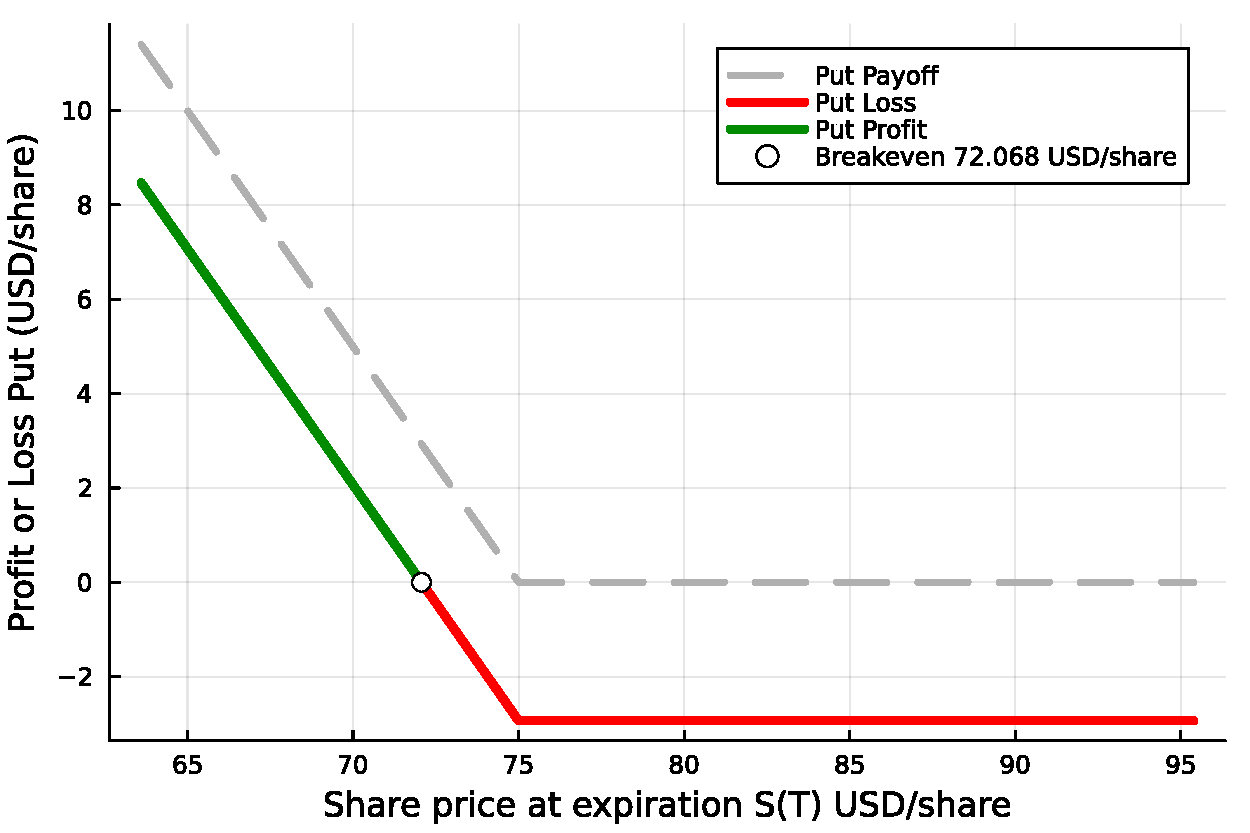
\includegraphics[width=0.65\textwidth]{./figs/Fig-Example-Put-K75-62DTE.pdf}
    \caption{Schematic of the payoff, profit and breakeven for a \texttt{long call} 
	contract. The gray dashed line denotes the payoff at expiration for the buyer.
	The red line denotes share prices at expiration that result in a loss for the buyer, 
	while the green line denotes share prices at expiration that result in a profit for the buyer.
	Parameters: the \texttt{put} 
	contract strike price is $K$ = 75 USD/share and a midpoint of premium $\mathcal{P}_{c}$ = 2.93 USD/share.}\label{fig:put-payoff-profit-breakeven-diagram}
\end{figure}

\section*{Summary}
In this module we introduced American style \texttt{put} contracts.
A \texttt{put} contract gives the holder the right, but not the obligation, to sell an underlying asset at a specified price (strike) on or before a future date (expiration).
We introduced the payoff and profit diagrams for \texttt{put} contracts.



% \bibliography{References_v1}

\clearpage
\printindex

\end{document}
